\documentclass[12pt]{article}
\usepackage[margin=1in]{geometry}
\usepackage[T1]{fontenc}
\usepackage{mathptmx}
\usepackage{graphicx}
\usepackage{booktabs}
\usepackage{hyperref}
\usepackage{float}
\usepackage{xcolor}
\usepackage{titlesec}
\titlespacing*{\section}{0pt}{1em}{0.5em}
\usepackage{setspace}
\onehalfspacing
\setlength{\parindent}{0pt}
\setlength{\parskip}{6pt}
\graphicspath{{Figures/}{figures/}{./}}

\title{\textbf{Emotion Detection from Text with Explainable Predictions}\\
\date{}
\large Deliverable 1: Problem Definition \& Data Foundations\\[2pt]
\normalsize Track A -- Application Development}
\author{}
\begin{document}
\maketitle
\vspace{-6em}
\begin{flushleft}
\large
Annushay Fatima (24L-2585)\\
Gul E Zara (24L-2592)\\
Rumesha Naveed (24L-2603)
\end{flushleft}
\vspace{-1.5em}


\section*{Abstract}
We are building a web application that detects the emotion in short English text (sadness, joy, love, anger, fear, surprise) and highlights the words behind its prediction. This report covers Phase 1 (problem definition) and Phase 2 (data acquisition and preprocessing). We use the public \texttt{dair-ai/emotion} dataset, clean it, analyse it, and prepare the inputs for three models that will be compared in later phases: TF-IDF with Logistic Regression, a BiLSTM and a fine-tuned DistilBERT.

\medskip
\noindent \textbf{GitHub:} \url{https://github.com/l242585-ai/Emotion_Detector}
%------------------------------------------------------------
\section{Phase 1: Problem Definition}

\subsection{Problem Statement}
Online text such as product reviews, support chats and posts in mental-wellness apps carries emotional information that is difficult to read at scale. Classical sentiment analysis only separates positive from negative, which is too coarse: anger, fear and sadness are all ``negative'' but call for very different responses. This project classifies short text into six emotions and shows which words drove the prediction, so that a human reader can judge whether to trust the result.

\subsection{Target Audience}
\begin{itemize}
  \item Customer-support teams who need to prioritise angry or distressed customers.
  \item Content moderators who screen large volumes of user-written text.
  \item Developers of mental-wellness and journaling applications.
  \item Researchers: the project addresses the gap of \emph{explainable} emotion detection, where a model shows evidence for its label instead of only outputting it.
\end{itemize}

\subsection{AI Justification}
A rule-based or keyword approach breaks down quickly for this task. Negation (``I am not happy'') flips the emotion while keeping the keyword, sarcasm hides the real emotion, and the same word can express different emotions in different contexts. Writing rules for all such cases is not feasible. Machine learning models learn these patterns directly from labelled examples, and deep models can also use word order and context. By comparing a bag-of-words baseline (TF-IDF with Logistic Regression) against a BiLSTM and a transformer (DistilBERT), we can measure how much context-awareness improves results on this specific problem.

%------------------------------------------------------------
\section{Phase 2: Data Acquisition and Preprocessing}

\subsection{Data Collection}
We use the \texttt{dair-ai/emotion} dataset from Hugging Face (\url{https://huggingface.co/datasets/dair-ai/emotion}). The script \texttt{Data\_Scripts/01\_download\_data.py} downloads it with the \texttt{datasets} library and writes the three raw splits to \texttt{data/raw/} as CSV files with the columns \texttt{text} and \texttt{label}. The splits contain 16{,}000 training, 2{,}000 validation and 2{,}000 test samples. Labels are integers: 0 sadness, 1 joy, 2 love, 3 anger, 4 fear, 5 surprise. Raw and processed data are excluded from the repository through \texttt{.gitignore}; the scripts reproduce them.

\subsection{Data Cleaning}
The script \texttt{Data\_Scripts/02\_clean\_data.py} performs the following steps and prints the counts for each split:
\begin{enumerate}
  \item \textbf{Missing values:} the number of missing values in each split is checked.
  \item \textbf{Duplicates:} duplicate texts are removed within each split (\texttt{drop\_duplicates} on the \texttt{text} column).
  \item \textbf{Text-length outliers:} the length of each text in words is computed and outliers are removed with the interquartile-range (IQR) rule. For each split the bounds are $Q_1 - 1.5\,\mathrm{IQR}$ and $Q_3 + 1.5\,\mathrm{IQR}$, and samples outside the bounds are removed.
  \item \textbf{Train/validation/test leakage check:} after cleaning, the overlap between the sets of texts of the three splits is counted for every pair of splits.
  \item \textbf{Saving:} cleaned files are written to \texttt{data/processed/} as \texttt{train\_cleaned.csv}, \texttt{val\_cleaned.csv} and \texttt{test\_cleaned.csv}.
\end{enumerate}
Punctuation is not removed during cleaning. Lowercasing is applied later by the TF-IDF vectoriser and in the EDA word statistics.

Table~\ref{tab:cleaning} summarises the effect of cleaning. In total, 406 training samples (2.5\%), 42 validation samples and 23 test samples were removed. \textcolor{red}.

\begin{table}[H]
\centering
\caption{Dataset size before and after cleaning.}
\label{tab:cleaning}
\begin{tabular}{lrrr}
\toprule
 & Train & Validation & Test \\
\midrule
Rows before cleaning & 16{,}000 & 2{,}000 & 2{,}000 \\
Missing values found & 0 & 0 & 0 \\
Duplicates removed & 31 & 2 & 0 \\
Length outliers removed & 375 & 40 & 23 \\
\midrule
Rows after cleaning & 15{,}594 & 1{,}958 & 1{,}977 \\
Total removed & 406 & 42 & 23 \\
\bottomrule
\end{tabular}
\end{table}

The leakage check reports the overlap for train--validation, train--test and validation--test as 5, 11 and 3 texts respectively \textcolor{red}.

\subsection{Exploratory Data Analysis}
The charts below are produced by \texttt{Data\_Scripts/03\_eda.py} from the cleaned data and saved in the \texttt{Figures/} folder.

\paragraph{Class distribution.}
Figure~\ref{fig:classes} shows that the dataset is clearly imbalanced. In the cleaned training set, joy (5{,}233 samples, 33.6\%) and sadness (4{,}557, 29.2\%) make up about 63\% of the data, while surprise has only 552 samples (3.5\%). The ratio between the largest and the smallest class is about 9.5$\times$. Validation and test sets show the same pattern, so the imbalance is consistent across splits. Because accuracy would be dominated by joy and sadness, we will evaluate models with \textbf{macro-F1} and use class weights during training.

\begin{figure}[H]
  \centering
  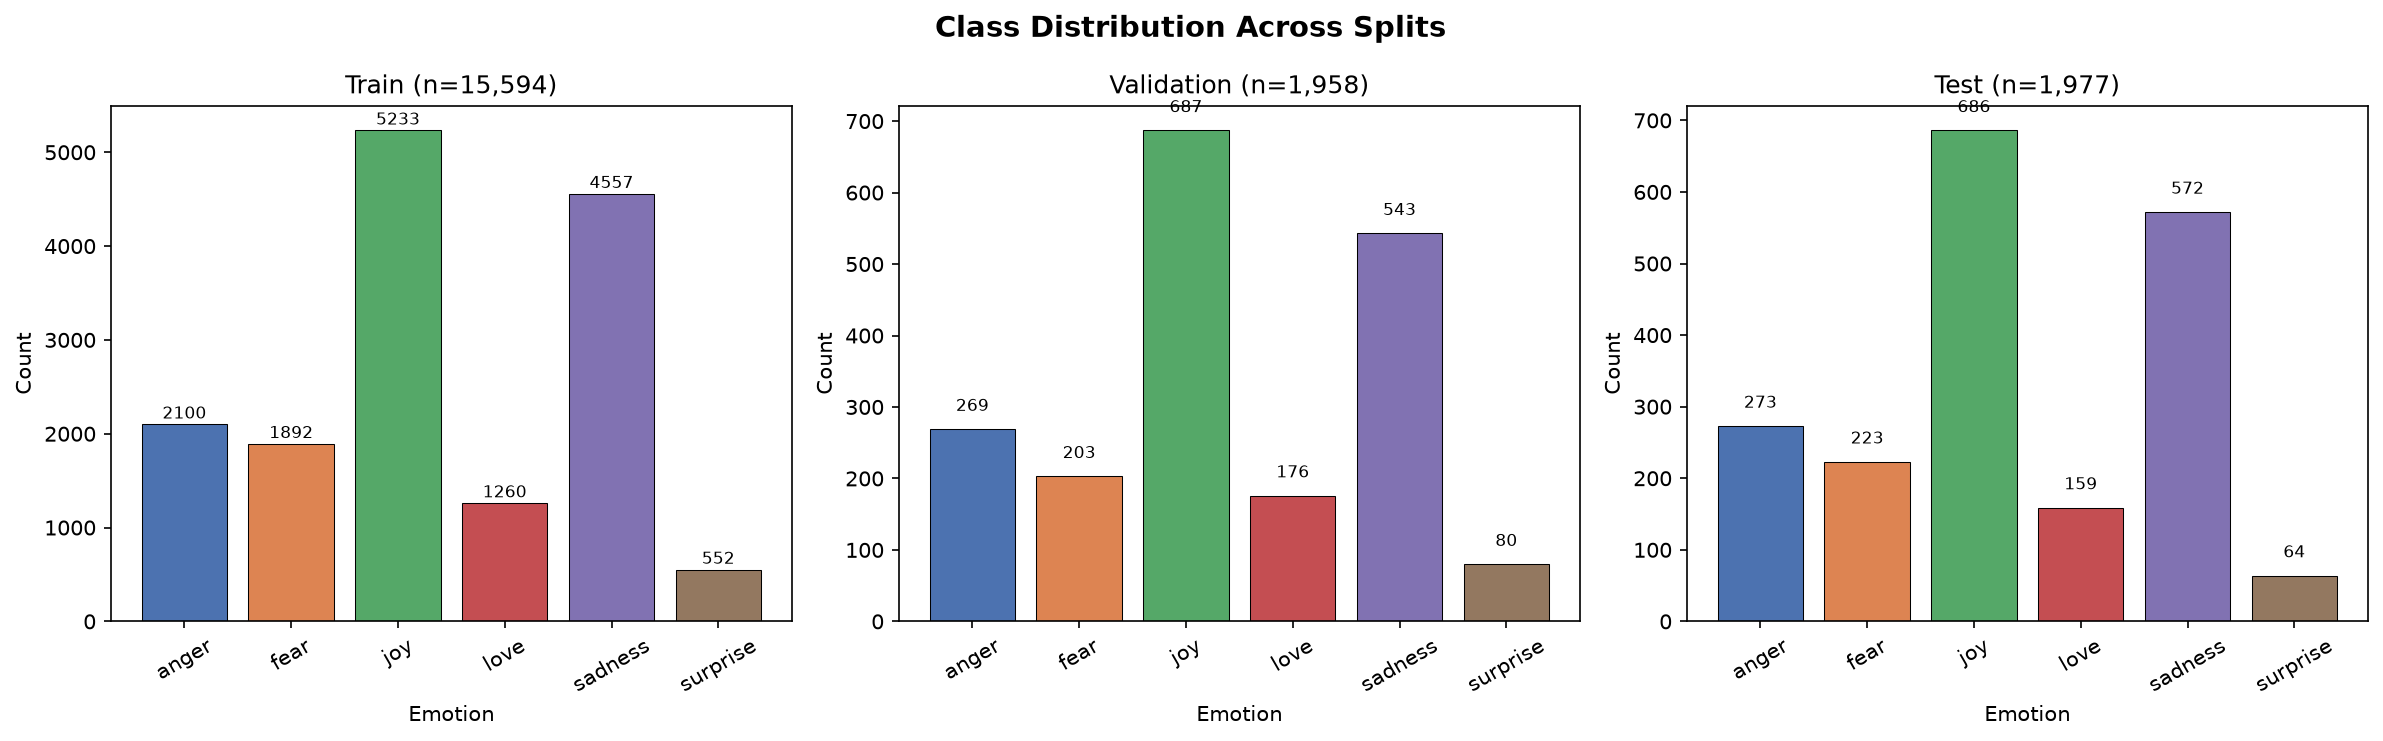
\includegraphics[width=\textwidth]{01_class_distribution.png}
  \caption{Class distribution of the cleaned train, validation and test splits.}
  \label{fig:classes}
\end{figure}

\paragraph{Text length.}
Figure~\ref{fig:length} shows that texts are short and right-skewed: most contain between about 5 and 25 words, with a long tail up to roughly 45 words after outlier removal. The length distributions of the six emotions overlap strongly, so text length alone is a weak signal and the models have to rely on the actual words.

\begin{figure}[H]
  \centering
  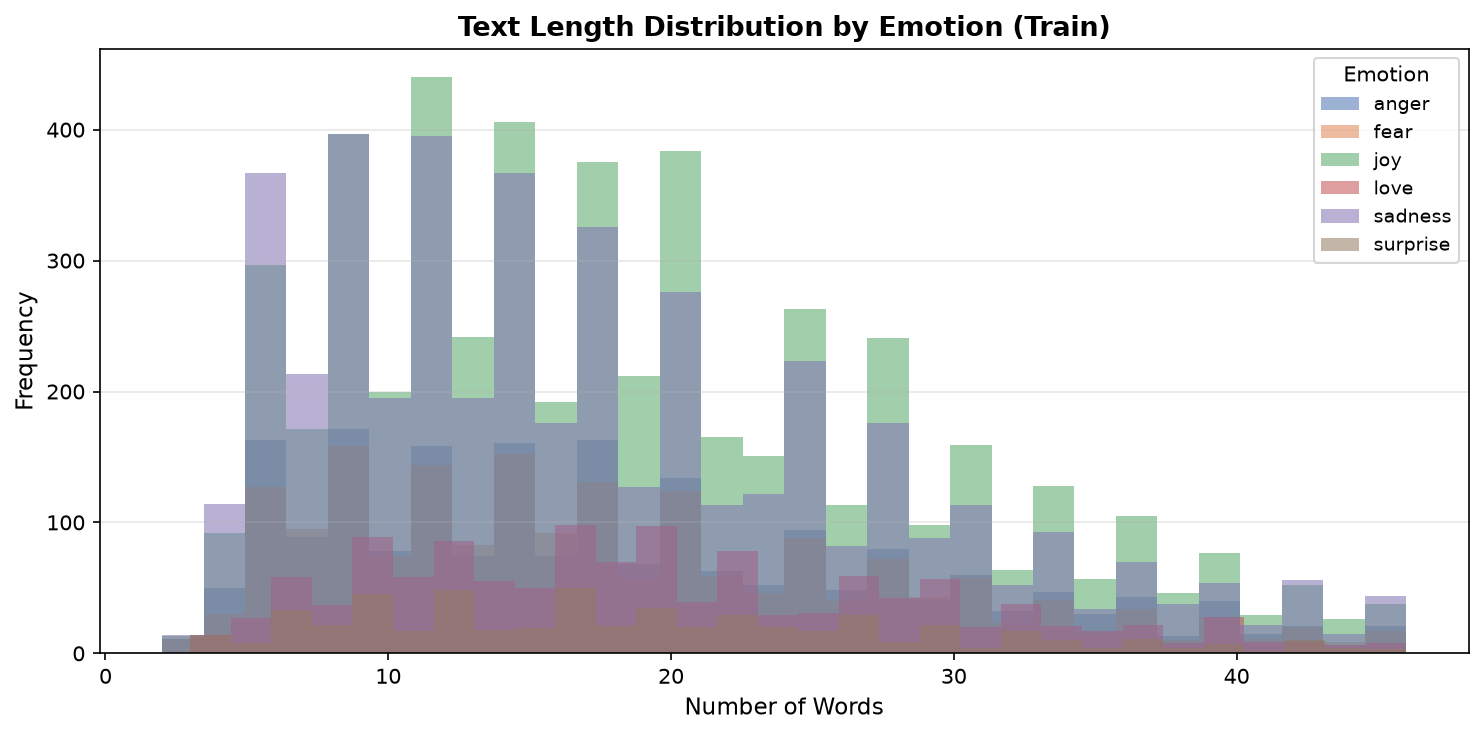
\includegraphics[width=0.9\textwidth]{02_text_length_distribution.png}
  \caption{Text length (number of words) by emotion, training set.}
  \label{fig:length}
\end{figure}

\paragraph{Word clouds and top words.}
Figures~\ref{fig:clouds} and~\ref{fig:topwords} show the most frequent words per emotion after removing stop words. The word clouds contain clear emotion words: for example \emph{irritable}, \emph{offended} and \emph{angry} for anger, \emph{nervous}, \emph{terrified} and \emph{afraid} for fear, \emph{loving} and \emph{caring} for love, and \emph{amazed}, \emph{impressed} and \emph{overwhelmed} for surprise. The raw frequency bar charts, however, are dominated by generic words such as \emph{because}, \emph{all}, \emph{more} and \emph{can}, which appear in almost every class. Only surprise and love have strongly distinctive top words. This shows that raw word counts are not enough to separate the emotions and motivates the use of TF-IDF weighting and context-aware models. The word clouds also contain a few offensive words that come directly from the source data.

\begin{figure}[H]
  \centering
  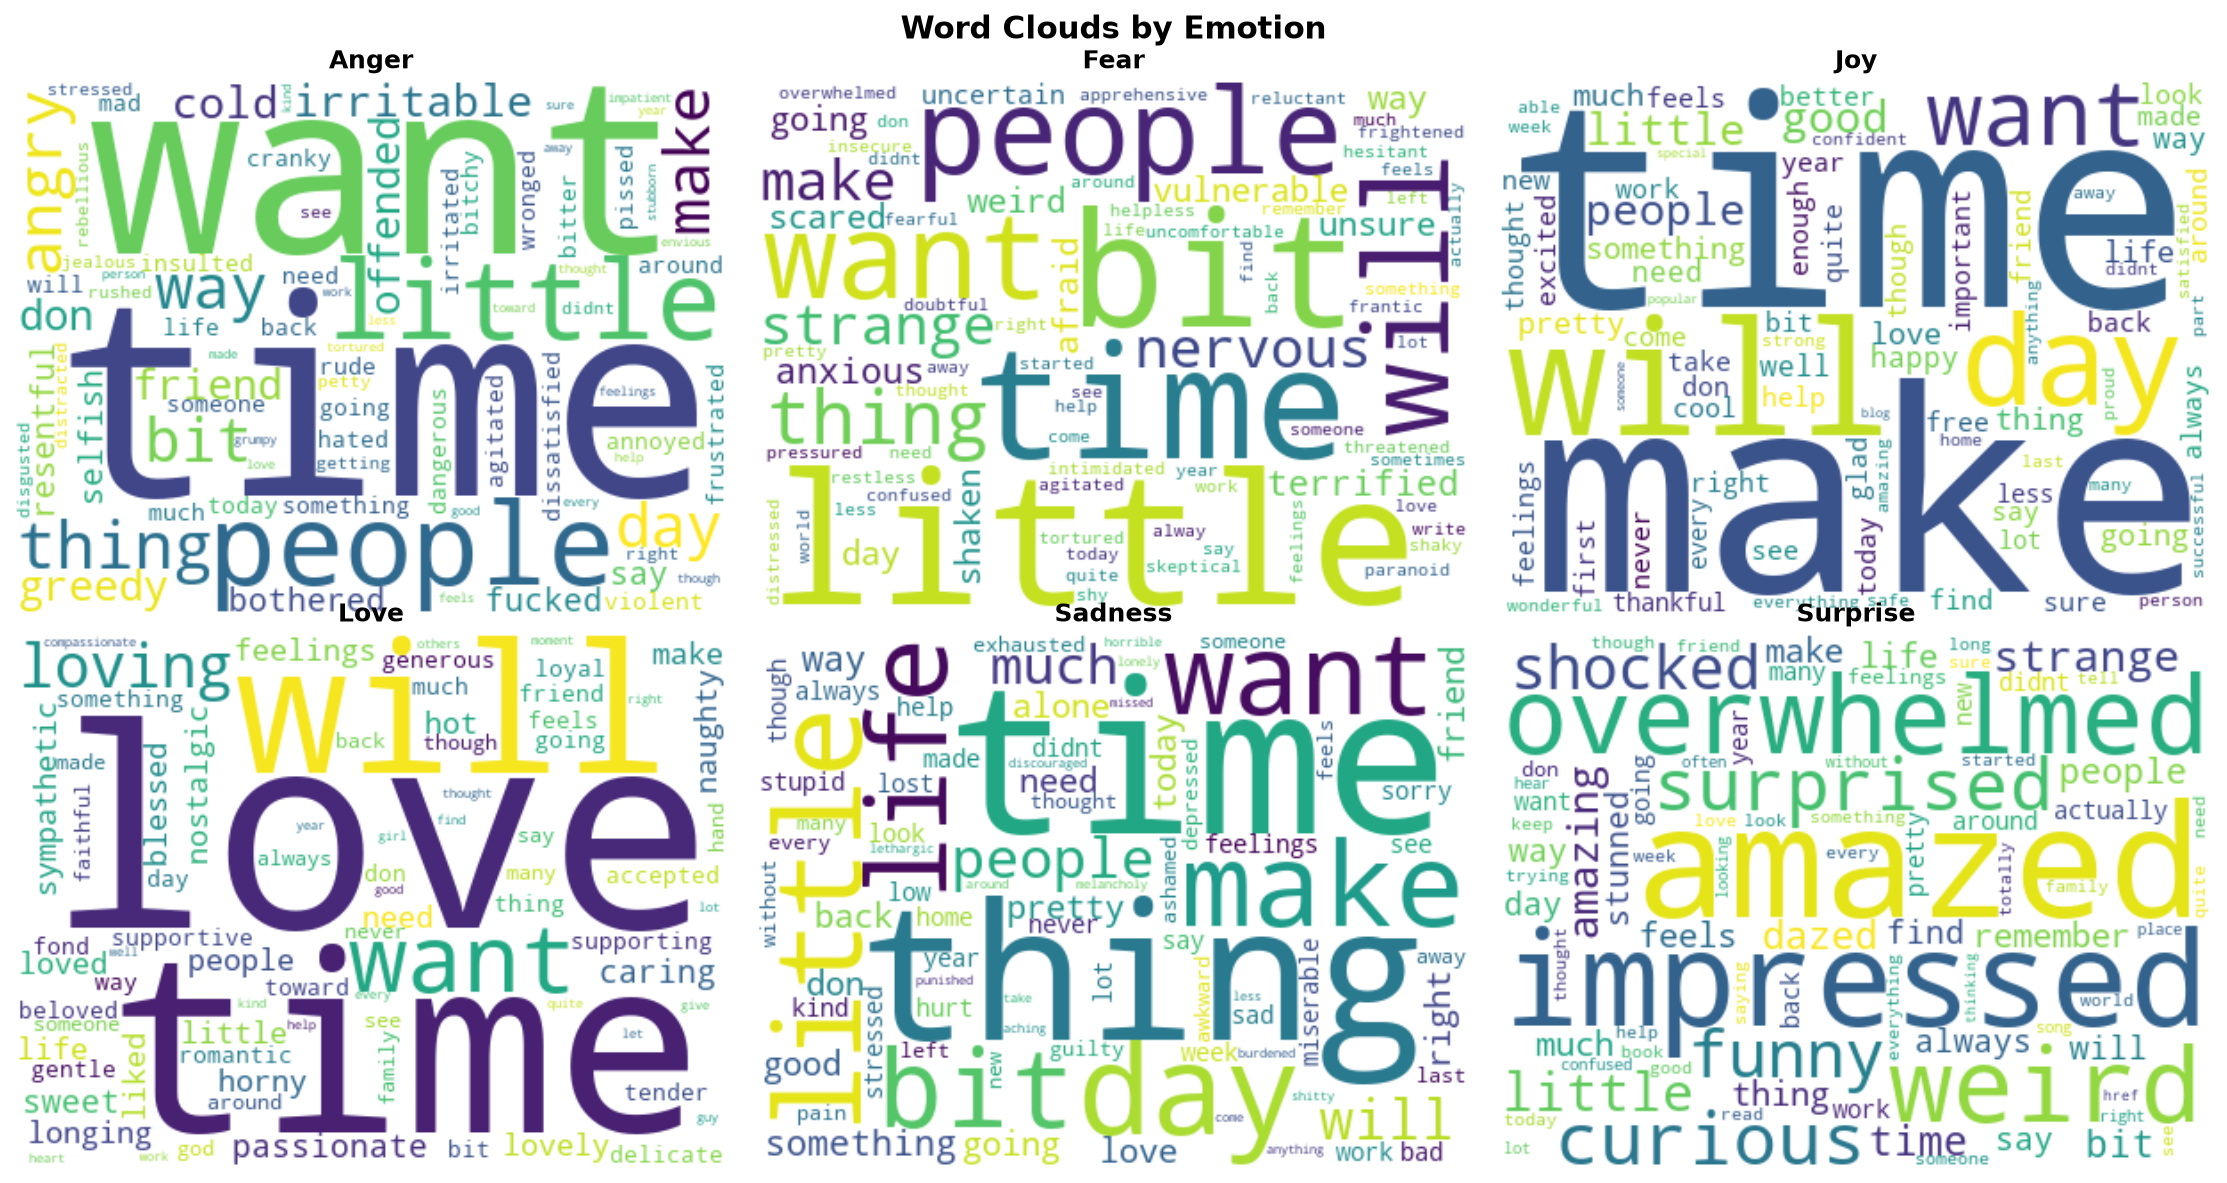
\includegraphics[width=\textwidth]{03_word_clouds.png}
  \caption{Word clouds per emotion (training set, stop words removed).}
  \label{fig:clouds}
\end{figure}

\begin{figure}[H]
  \centering
  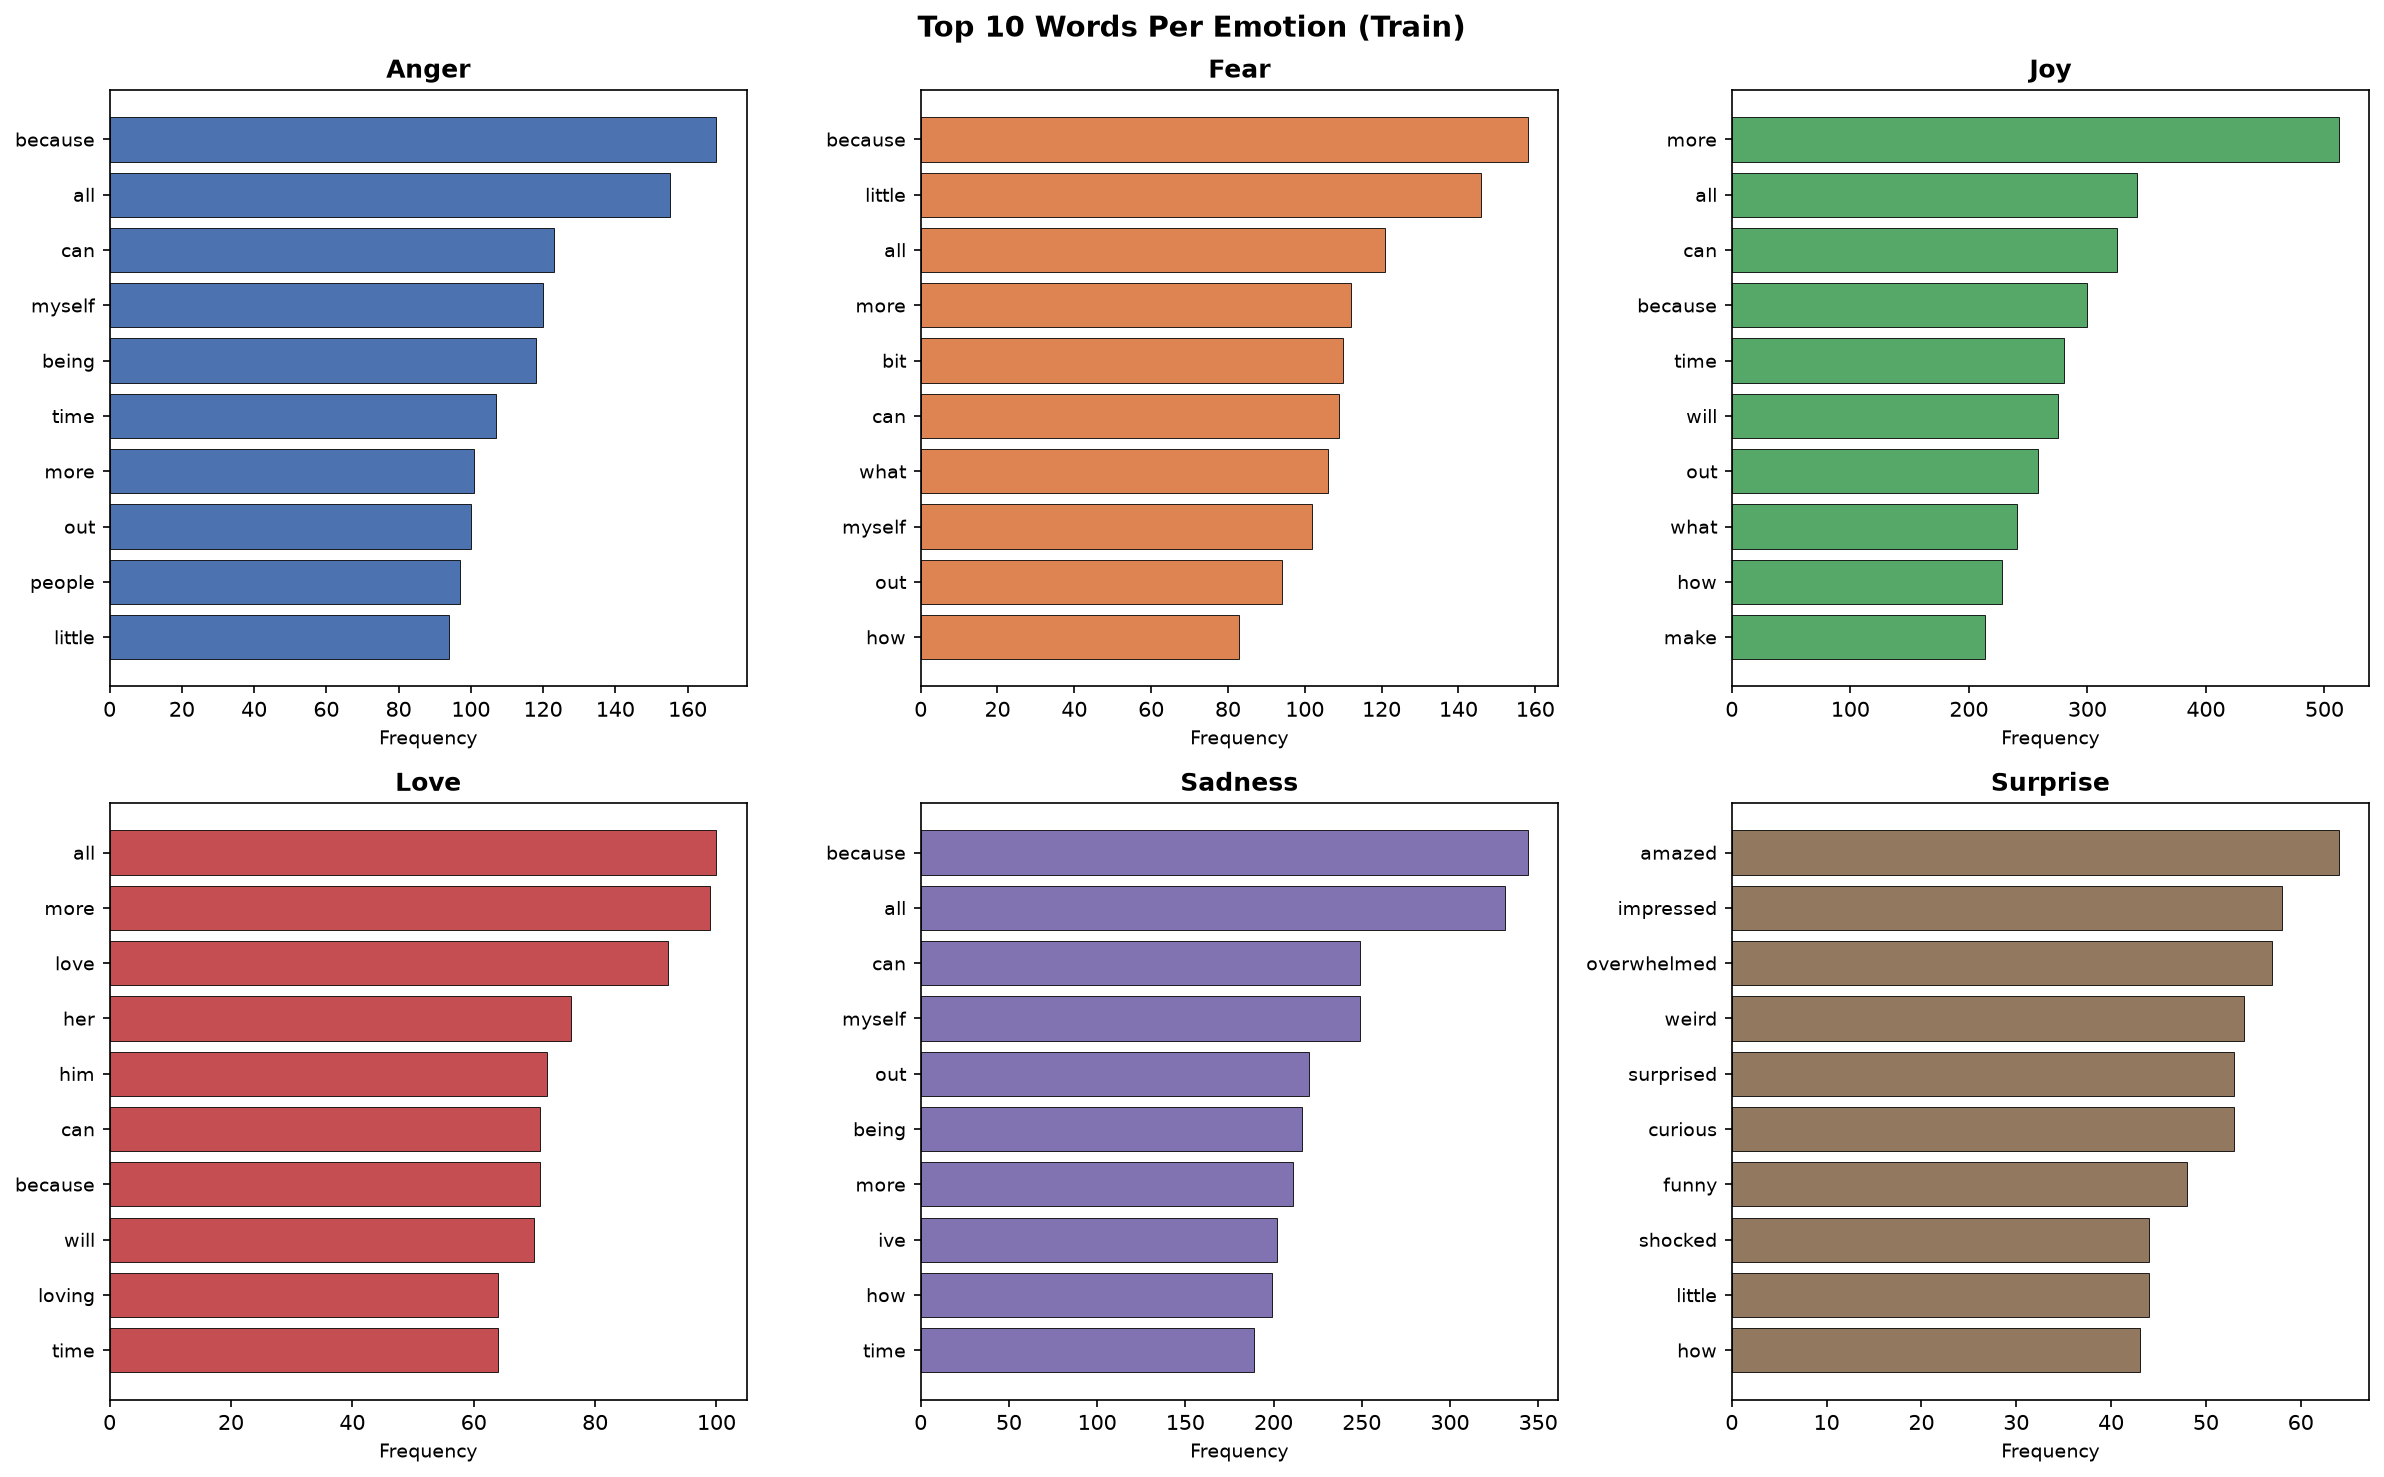
\includegraphics[width=\textwidth]{04_top_words_per_emotion.png}
  \caption{Ten most frequent words per emotion (training set, stop words removed).}
  \label{fig:topwords}
\end{figure}

\paragraph{Distribution across splits.}
Figure~\ref{fig:heatmap} compares the share of each emotion in the three splits. The proportions are almost identical, so the validation and test sets are representative of the training data. Note that this heatmap shows label proportions per split and not correlations between numeric features; the dataset consists of raw text, so no numeric feature columns exist before feature extraction.

\begin{figure}[H]
  \centering
  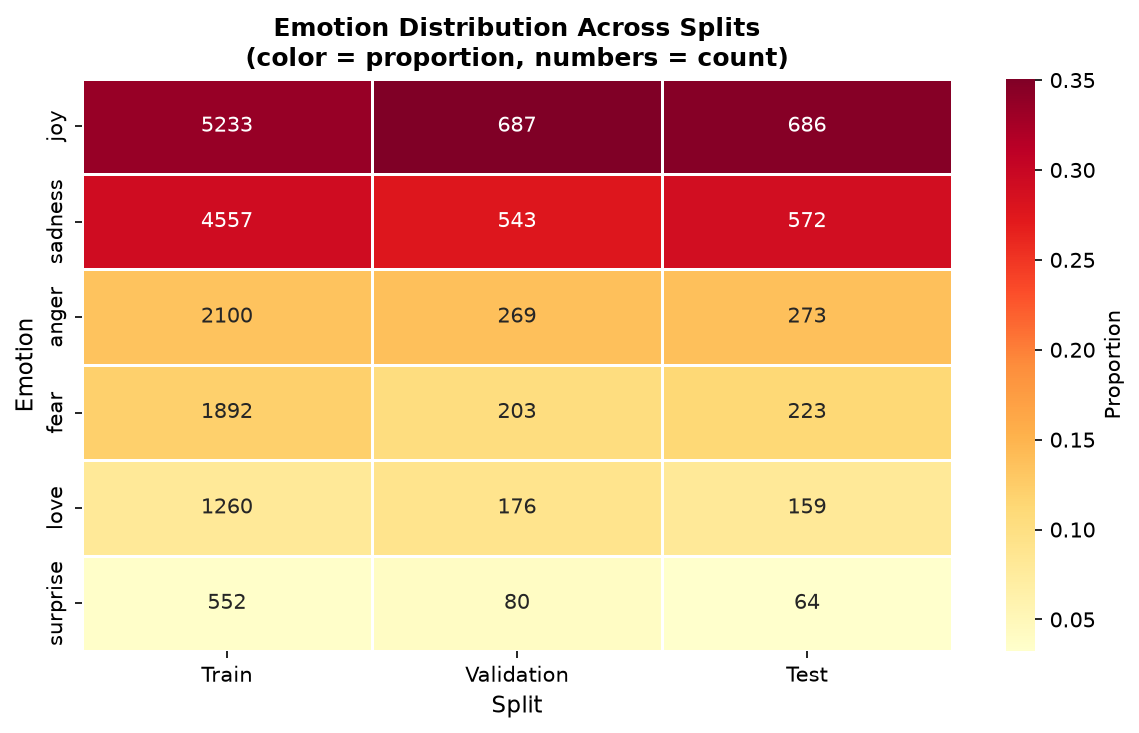
\includegraphics[width=0.75\textwidth]{05_emotion_split_heatmap.png}
  \caption{Emotion distribution across splits (colour = proportion, numbers = counts).}
  \label{fig:heatmap}
\end{figure}

\subsection{Feature Strategy}
The script \texttt{Data\_Scripts/04\_features.py} prepares the inputs for the three planned models from the cleaned data. All vectorisers are fitted on the training set only and then applied to validation and test data, which avoids leakage from evaluation data.

\begin{itemize}
  \item \textbf{Encoding of labels.} Labels are the integers 0--5 (Section~2.1). A scikit-learn \texttt{LabelEncoder} over the emotion names is saved for decoding predictions later.
  \item \textbf{TF-IDF features (Logistic Regression baseline).} \texttt{TfidfVectorizer} with unigrams and bigrams, at most 20{,}000 features, \texttt{min\_df}$=3$, \texttt{max\_df}$=0.95$, sublinear term frequency (logarithmic scaling), Unicode accent stripping, and a token pattern that keeps only alphabetic words of at least two letters. Text is lowercased by the vectoriser, and each row is L2-normalised by default, which is the normalisation step for this feature type. The resulting sparse matrices are saved as \texttt{.npz} files together with the fitted vectoriser. The actual vocabulary size is 18,106 \textcolor{red}.
  \item \textbf{Tokenisation and padding (deep models).} The \texttt{distilbert-base-uncased} tokenizer converts each text into subword token IDs and an attention mask, truncated or padded to a fixed length of 128 tokens. These arrays are saved for the DistilBERT fine-tuning and can also be used as padded integer sequences for the embedding layer of the BiLSTM. If the \texttt{transformers} library is not installed, the script falls back to a simple word-index vocabulary of up to 10{,}000 words with the same fixed length.
  \item \textbf{Scaling.} We do not add hand-crafted numeric features such as text length, because the EDA showed that length differs little between emotions. Normalisation is therefore handled by the L2-normalised TF-IDF vectors; for the neural models the inputs are integer token IDs, which are not scaled.
  \item \textbf{Class imbalance.} Balanced class weights $w_c = n / (k \cdot n_c)$ are computed from the training labels, with $n=15{,}594$ samples and $k=6$ classes (Table~\ref{tab:weights}), and saved for use in model training. Rare classes receive larger weights.
\end{itemize}

\begin{table}[H]
\centering
\caption{Class weights computed from the cleaned training set.}
\label{tab:weights}
\begin{tabular}{llrr}
\toprule
Label & Emotion & Train samples & Weight \\
\midrule
0 & sadness  & 4{,}557 & 0.570 \\
1 & joy      & 5{,}233 & 0.497 \\
2 & love     & 1{,}260 & 2.063 \\
3 & anger    & 2{,}100 & 1.238 \\
4 & fear     & 1{,}892 & 1.374 \\
5 & surprise &   552   & 4.708 \\
\bottomrule
\end{tabular}
\end{table}

%------------------------------------------------------------
\section{Team Contributions}
\begin{itemize}
  \item \textbf{Annushay Fatima:} repository setup, folder structure, data download script, README, project description sections of the report.
  \item \textbf{Gul E Zara:} data cleaning and validation script, task division, cleaning section of the report.
  \item \textbf{Rumesha Naveed:} exploratory data analysis, feature engineering scripts and all figures.
\end{itemize}

\section{Conclusion and Next Steps}
We defined the problem, justified the use of machine learning, collected the \texttt{dair-ai/emotion} dataset, cleaned it, analysed it and prepared the features for all three planned models. The main data challenge is the strong class imbalance (about 9.5$\times$ between joy and surprise), which we address with macro-F1 evaluation and class weights. The next phases are training and comparing the TF-IDF + Logistic Regression, BiLSTM and DistilBERT models on macro-F1, latency and bias, adding word-level explanations, and deploying the best model behind an API with a Streamlit interface.

\end{document}